\section{Results/Analysis}

\subsection{Comparison between frameworks}
To compare between CNN frameworks, AlexNet was trained for many iterations on each framework.
The whole process was profiled, and one mini-batch iteration was selected for analysis after the time metrics were stabilized.
Model parameters and hyperparameters of the solver are carefully equalized previously in order to remove the effect from things other than the framework itself.
The result is shown in Figure~\ref{}.

First, we focused at how each framework chose kernels.
Caffe did not provide any user options to affect kernel choices.
Instead, Caffe depended on cuDNN's heuristics, which try to determine the best suited algorithm under the given specification.
Surprisingly, Caffe did not have appropriate memory strategy for kernels yet, just passing 8MB workspace limit as an argument.
Low-memory required algorithms, such as gemm and winograd, were selected, resulting in low performance compared to other frameworks.
Tensorflow also did not provide options for kernel choices.
Unlike Caffe, however, it executed all available algorithms on the first run by itself.
Only the fastest kernels in each layer were executed for subsequent runs.
Under the AlexNet, FFT algorithms were chosen for all convolution layers except the first layer, where FFT cannot be used due to stride of 4.
One downside was that algorithms were chosen from hardcoded set, so recently added option (like WINOGRAD\_NONFUSED) was not included.
On the other hand, Theano provide full access on the kernel choices.
We could specify convolution algorithms to be used, globally or layer-by-layer.
We found layerwise option is better, since implicit gemm is chosen as fallback if the layer specification does not match global option, and it can even be slower than explicit gemm which is the default option.
%TODO see first layer of theano fft
Theano also had 'guess\_once' option, which depended on cuDNN's heuristics like Caffe but provided proper arguments.
'time\_once' option was provided, too, which depended on cuDNN's functionality that run all available convolution algorithms and chose the fastest one.
Theano did not have downside like TensorFlow had, because it directly used cuDNN's API.
If 'time\_once' option was on, it used gemm on the first layer and had mixed use of FFT and winograd on the rest convolution layer.
When 'guess\_once' option was on, it used slightly different kernels but showed almost identical running time with 'time\_once' option, proving that heuristic of cuDNN is quite reliable.
Although Theano executed the fastest convolution kernels, Theano did not have the fastest convolution when it came to the whole layer.
Theano used its own runtime-compiled kernels for bias add and ReLU activation, and they were more than twice slower than cudnn's or other libraries'.
%TODO table needed
Torch provided full control on the kernel choices, similar to Theano.
Torch's cuDNN backend, cudnn.torch had cudnn.benchmark option which is the same with 'time\_once' in Theano.
When benchmark option is on, Torch showed overall fastest execution time among four frameworks.

We also found a few phenomenons in terms of framework overhead.
The most noticable one was the tensor format.
Caffe, Theano, and Torch used NCHW tensor format, which means (batch, channel, height, width) dimensions.
Tensorflow supported NCHW, but it used NHWC more popularly.
Its tutorial codes used NHWC format, and many functions, like conv2d, used NHWC as a default argument.
While NHWC can be faster when there are channel-wise operations, some cuDNN's convolution kernels (such as FFT) only support NCHW format.
Besides, TensorFlow always do NHWC-to-NCHW dimension swap even if it is using NHWC-supported kernels.
Therefore, using NHWC tensor format leads to intensive dimension swapping before and after the convolution.
In our AlexNet, just changing tensor format from NHWC to NCHW led to about 15\% improve in speed on TensorFlow.
Second issue was backward data convolution in the first convolution layer.
The first layer does not have previous layer to update parameters, so it does not need backward data convolution, which basically calculates output gradients for the previous layer.
Caffe and Theano automatically did not execute the operation, and it can be disabled by setting gradInput of the first layer to nil.
On TensorFlow, however, we did not find any option to disable the operation through train.MomentumOptimizer, leading to slow backward pass in the first layer.

%그 외 사소한 것으로 텐서에 네트워크 입력을 feed_dict로 주면 CPU 복사가 일어나서 매우 느리므로 FixedLengthRecordReader 등으로 주는게 좋다.
%https://github.com/tensorflow/tensorflow/issues/2919

%https://github.com/BVLC/caffe/blob/rc3/src/caffe/layers/cudnn_conv_layer.cpp#L113
%https://github.com/tensorflow/tensorflow/blob/v0.10.0rc0/tensorflow/core/kernels/conv_ops.cc#L460
%https://github.com/tensorflow/tensorflow/blob/v0.10.0rc0/tensorflow/stream_executor/cuda/cuda_dnn.cc#L933
%https://github.com/Theano/Theano/blob/rel-0.8.2/theano/sandbox/cuda/dnn.py#L285
%https://github.com/Theano/Theano/blob/rel-0.8.2/theano/sandbox/cuda/dnn_fwd.c#L227
%https://github.com/soumith/cudnn.torch/blob/R5/SpatialConvolution.lua#L166

\subsection{characterization of different convolution algorithms}
Since forward and backward propagation of convolution layers takes most of the running time, we run the same model on different convolution kernel to characterize the performance of each convolution algorithm.
Three types of convolutions are computed for each iteration.
forward convolution(FWD) computes the layer output, backward data convolution(BD) computes backward gradient input and backward filter convolution(BW) computes gradients of network parameters.
CuDNN R5 supports matrix multiplication convolution(gemm), FFT convolution, and winograd convolution.
CuDNN has various gemm convolution algorithms and the tested algorithm is implicit gemm precomp algorithm.
Winograd convolution cannot be applied to BW convolution on CuDNN 5.0 hence we use fft convolution instead.(CuDNN 5.1RC supports winograd nonfused option)
Since the first convolution layer has stride of 4, Winograd and FFT convolution cannot be applied.
Direct convolution is tested by Torch binding of Cuda-convnet3.
All comparisons are done on Torch 7 because Torch can specify convolution algorithm on each layer and newest version of Cuda-convnet3 is only supported by Torch7.

Randomly generated batch inputs are used to remove IO latency.
The forward and backward propagation time is measured as average of 100 iterations.
The compute times and statistics of kernels are measured by NVIDIA nvprof profiler.
The theoretical floating point operation counts are calculated as 2 * K*CRR*NWW since each calculation uses 1 addition and 1 multiplication.
We compare them to actual floating-point operation counts of the kernels.
Flops of the kernels are calculated as Flop count/execution time.
FFT convolution consists of 2 FFTs and 1 complex matrix multiplication, thus statistics of those 3 kernels are added together.

\begin{figure}
  \centering
  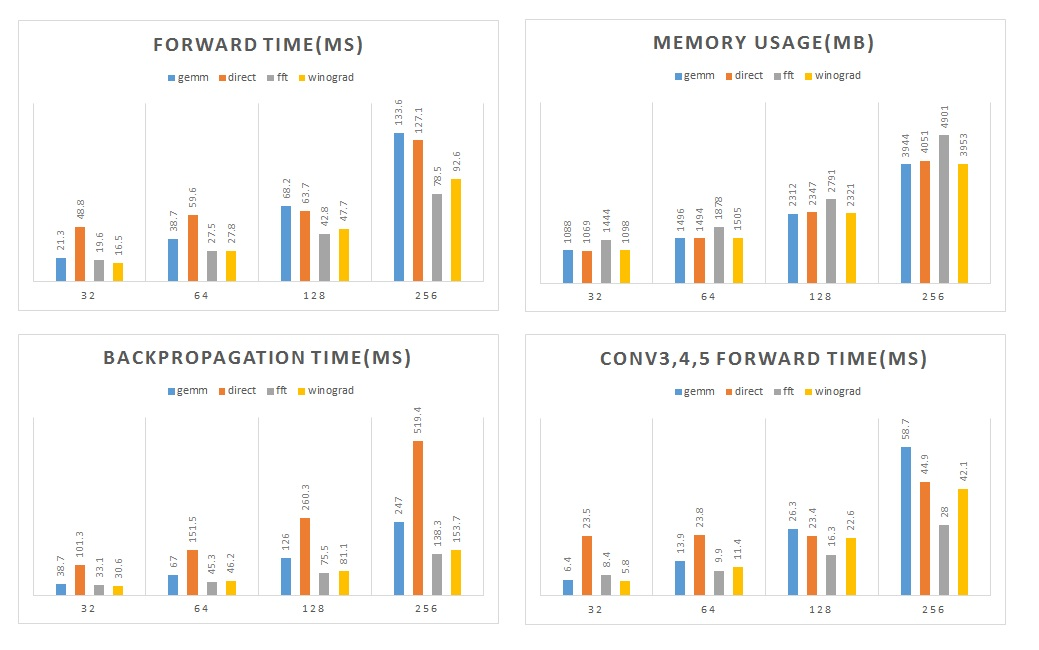
\includegraphics[width=\linewidth]{./figures/conv_time}
  \caption{Forward propagation and Backpropagation times of convolution algorithms. The times are measured as average of 100 batch iterations. 
Direct convolution is tested with cuda-convnet3 and other 3 are kernels of CuDNN R5. }
  \label{fig_conv_time}
\end{figure}

FIg \ref{fig_conv_time} shows execution time comparisons between convolution kernels.
Winograd convolution and FFT convolution always perform better than direct or gemm convolution, due to smaller floating point operations required.
FFT has smallest operations count, makes it fastest among algorithms on big batch inputs.
However FFT scales bad on smaller batch sizes because it executes 5 kernels per each layer.
The forward propagation speed comparison on conv layer 3,4,5 on (f) of Fig \ref{fig_conv_time} clearly shows the differences.
Cuda-convnet scales bad when the batch size is smaller than 128 while GEMM convolutoin sclaes almost linearly.
Winograd performs better when the batch size is smaller than 64, where theoretical operations per each layer is around 20G operations.
Winograd kernels are more efficient when the sample width is even.
When we increase the sample width of conv layer 3,4,5 from 13 to 14, the execution time of Winograd kernels decrease by 10\%.

Number of floating point operations needed for forward propagation and backward propagation kernels are equal on the same layer.
Therefore, execution time of forward and backward propagation kernels are almost symmetric on most convolution algorithms.
However, backpropagation kernels of direct convolution takes more execution time than their forward counterparts.
Especially backward filter convolution on first convolution layer takes 200ms to execute, occupying 40\% of total training time.
The reason for the slow execution is low parallelism of kernels.
The backward direct convolution kernels have small thread numbers compared to other algorithms, generating 6 times smaller thread grid size.
The backward filter convolution for the first layer generates only 1024 threads, while Titan X has 3072 CUDA cores.





\begin{figure}
  \centering
  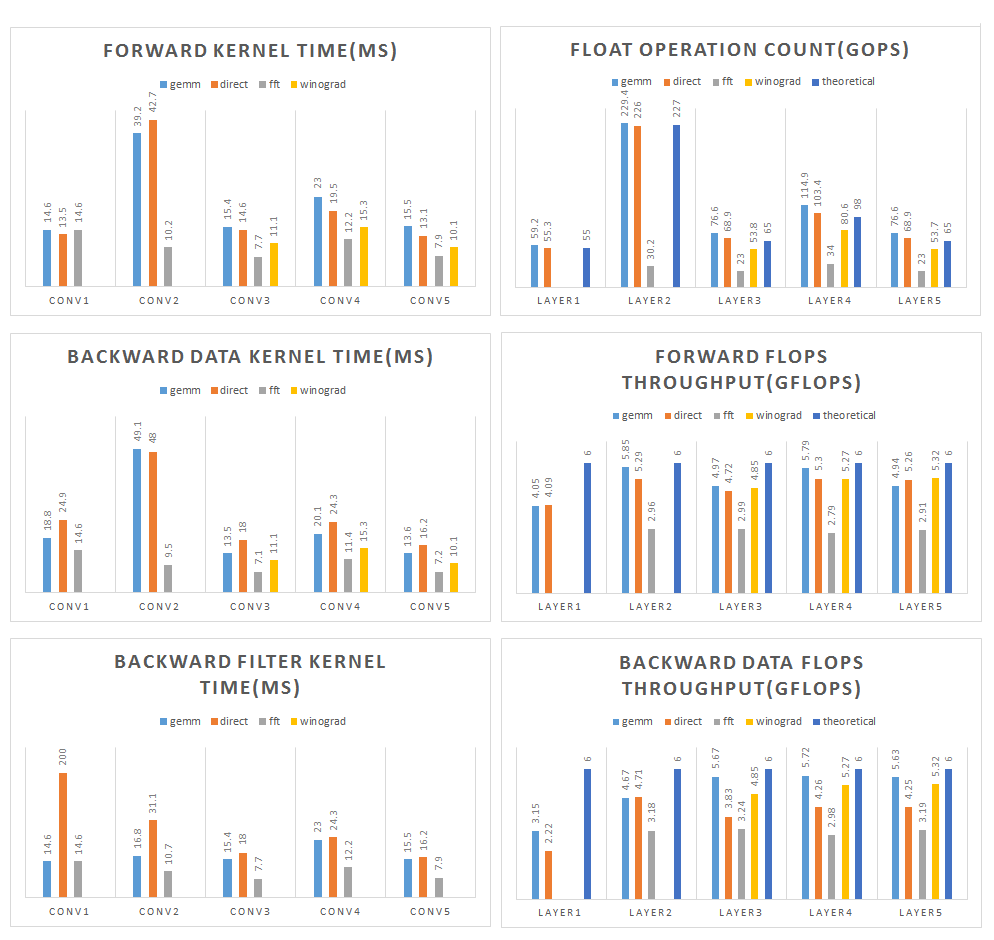
\includegraphics[width=\linewidth]{./figures/layerwise_bench}
  \caption{Layerwise analysis of convolution kernels}
  \label{fig_layerwise}
\end{figure}


\subsection{Multi GPU analysis}

\begin{itemize}
  \item Support
  \item Scalability : proportion of data exchange
  \item Synchronization cost
\end{itemize}

\section{Discussion / Conclusion}

\begin{itemize}
  \item Summary of results
  \item Compare frameworks : Implementation difference
  \item Locate bottleneck / suggest possible optimization
  \item Limitation, future research
\end{itemize}
